%こねこ。のテンプレート(ver 2.3)
%Copyright © 2021-2022 こねこ。 All Rights Reserved.

\documentclass[a4paper, 9pt]{jsarticle}
\usepackage[top=20truemm, bottom=20truemm, left=20truemm, right=20truemm]{geometry}

\usepackage{preamble}
%日本語を使うときは必須
\usepackage{jpreamble}
%化学用追加パッケージ
\usepackage{prechemistry}
%情報用追加パッケージ
\usepackage{preprog}
%フォント操作用追加パッケージ
\usepackage{prefonts}

\title{\sf{Activity Report 01}}
\author{\sf{回路班 首藤 朗}}
\date{\sf{\today}}
\begin{document}
\maketitle
\section{作成したもの}
LED点滅回路を,制御するプログラムを変更して作成した.500\ut{ms}ごとに4つのLEDが点滅する回路であり,PICマイコンをはじめマイコンを初めて扱う際によく扱われる回路のひとつである.
\section{作成した回路}
\fig{LED点滅回路の回路図}{fig1}{0.5}{test.pdf}
\newpage
\section{プログラム}
\lstinputlisting{LEDTimer.c}
\section{実際の写真}
\fig{未点灯時}{fig1}{0.08}{img1.jpg}
\fig{点灯時}{fig1}{0.08}{img2.jpg}

\section{手順}
まず,参考文献\cite{PIC}を参照しながら回路を作成した.この際,本回路はISCP接続を行い,PICマイコンをブレッドボードに埋め込んだ状態からPICKIT4へと配線を伸ばす方針とした.LEDは参考文献\cite{PIC}の中では黄色のものを用いていたが,手持ちが赤であったので赤のものを使用した.ジャンパは秋月電子のPIC書き込みアダプタに付属していたものを使用した.\par
次に,参考文献\cite{PIC}を参照しながら,MPLABを用いてプログラムを行なった.Configrationは本書に倣いMCCを使用せず,Configuration Bitsを用いて直接設定した.\par
書き込みはMPLABの書き込み機能を用い,さらに秋月電子のISCP対応PIC書き込みアダプターキットを用いて行なった.
\section{考察・感想}
今度はISCP(In-Circuit-Serial-Programming)接続を用いて開発を行った.今回,ブレッドボード上の容量の関係からスイッチをつけていないので,S1の挙動を試すために\tt{if(S1\_GetValue() = a)}の$a$の値を1にしてみたり,0にしてみたりしたが,確かに挙動が変化した.タイマーの割り込み処理を用いて,待ち時間の間に他の処理を実行する仕組みである.



\begin{thebibliography}{99}
	\bibitem{PIC} 後閑哲也,"逆引きPIC電子工作やりたいこと事典"(技術評論社,東京,2019),pp.48-49
\end{thebibliography}
\end{document}

%%%%%%%%%%%%%%%%%%%%%%%%%%%%%%%%%%%%%%%%%%%%%%%%%%%%%%%%%%%%%%%%%%%
%%%%%%%%%%%%%%%%%%%%%%%%%%%%%%%%%%%%%%%%%%%%%%%%%%%%%%%%%%%%%%%%%%%%%%%%%%%%%%%%%%%%%%%%%%%%%%%%%%%%%%%%%%%%%%%%%%%%%%%%%%%%%%%%%%%%%%%%%%%%%%%%%%%%%%%%%%%%%%%%%%%%%%%%%%%%%%%%%%%%%%%%%%%%%%%%%%%%%%%%%%%%%%%%%%%%%%%%%%%%%%%%%%%%%%%%%%%%%%%%%%%%%%%%%%%%%%%%%%%%%%%%%%%%%%%%%%%%%%%%%%%%%%%%%%%%%%%%%%%%%%%%%%%%%%%%%%%%%%%%%%%%%%%%%%%%%%%%%%%%%%%%%%%%%%%%%%%%%%%%%%%%%%%%%%%%%%%%%%%%%%%%%%%%%%%%%%%%%%%%%%

簡単なTikZテンプレート
参考:https://math-note.xyz/latex/tikz/tikz-line/

\begin{tikzpicture}
 \draw[->,>=stealth,semithick] (-2,0)--(2,0)node[above]{$x$}; %x軸
 \draw[->,>=stealth,semithick] (0,-1)--(0,3)node[right]{$y$}; %y軸
 \draw (0,0)node[below right]{O}; %原点
 \draw (-1,0)node[below]{$-1$}; %点(-1,0)
 \draw (0,1)node[right]{$1$}; %点(0,1)
 \draw[samples=1000, very thick,domain=#1] plot(#2, {#3})node[right]{$y=#4$};
\end{tikzpicture}

%媒介変数
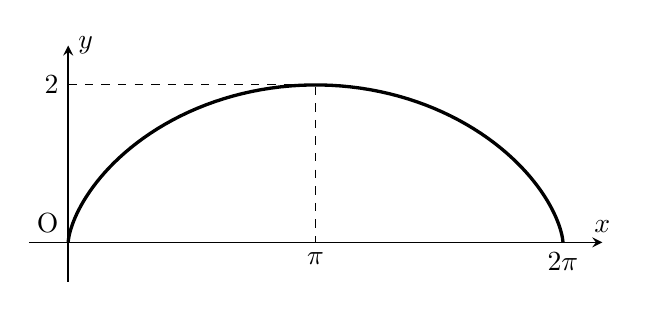
\begin{tikzpicture}
 \draw[->,>=stealth,semithick] (-0.5,0)--(2*pi+0.5,0)node[above]{$x$}; %x軸
 \draw[->,>=stealth,semithick] (0,-0.5)--(0,2.5)node[right]{$y$}; %y軸
 \draw (0,0)node[above left]{O}; %原点
\draw[very thick,samples=100,domain=0:2*pi,variable=\t] plot({\t-sin(\t r)},{1-cos(\t r)}); %サイクロイド%サイクロイド
 \draw (2*pi,0)node[below]{$2\pi$}; %点(2\pi,0)
 \draw[dashed] (0,2)node[left]{2}--(pi,2)--(pi,0)node[below]{$\pi$}; %点(\pi,2)
\end{tikzpicture}

%極座標
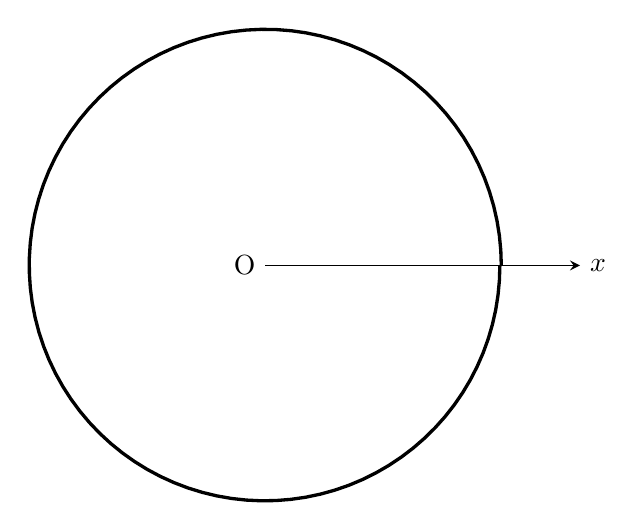
\begin{tikzpicture}
 \draw[->,>=stealth,semithick] (0,0)--(4,0)node[right]{$x$}; %始線
 \draw (0,0)node[left]{O}; %極
 \draw[very thick,samples=100,domain=0:2*pi,variable=\theta] plot(\theta r:{2*1.5*cos(\theta)}); %点(1.5,0)を中心とする半径1.5の円
\end{tikzpicture}

%円弧
\begin{tikzpicture}
 \draw[->,>=stealth,semithick] (-1.5,0)--(2.5,0)node[above]{$x$}; %x軸
 \draw[->,>=stealth,semithick] (0,-0.5)--(0,1)node[right]{$y$}; %y軸
 \draw (0,0)node[above left]{O}; %原点
 \draw (2,1)node[right]{A}; %点A(2,1)
 \draw[very thick] (2,1) arc (60:110:3); %点Aが偏角60度の点であるような半径3の円の,偏角60度から110度の部分の円弧
 \draw (2,1)++(60:-3)++(110:3)node[left]{B}; %円弧のAでない方の端点B(2,1)
\end{tikzpicture}

%複数グラフ
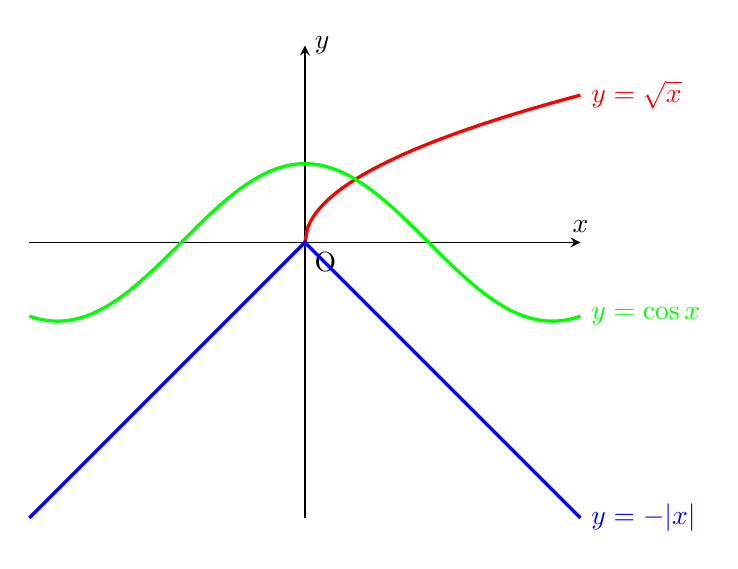
\begin{tikzpicture}
 \draw[->,>=stealth,semithick] (-3.5,0)--(3.5,0)node[above]{$x$}; %x軸
 \draw[->,>=stealth,semithick] (0,-3.5)--(0,2.5)node[right]{$y$}; %y軸
 \draw (0,0)node[below right]{O}; %原点
 \draw[red,very thick,samples=100,domain=0:3.5] plot(\x,{sqrt(\x)})node[right]{$y=\sqrt{x}$};
 \draw[blue,very thick,domain=-3.5:3.5] plot(\x,{-abs(\x)})node[right]{$y=-|x|$};
 \draw[green,very thick,samples=100,domain=-3.5:3.5] plot(\x,{cos(\x r)})node[right]{$y=\cos{x}$};
\end{tikzpicture}
